The platform target for this game is mobiles. The platform has some limitations in its input interface. The game being developed is a shooter(\ref{sec:selectionofgametype:mobiledevices}), which are fairly popular with large titles like \emph{Call Of Duty} and \emph{Battlefield}. These games can be played using a controller on consoles, and trying to recreate these controls on the touch interface will create a familiar input scheme with which players can relate.

\section{Gamepad Control Scheme}
Controlling the game with a gamepad is natively supported by Unity3D, where the user can use the Input Manager \cite{unity_manual_inputmanager} and add axes that use ''Joystick Axis''. Unity allows reading 20 different axes, where buttons also count as axes.

This is not straight forward however, if the game is to run on different platforms. It is even more difficult if the game should support different gamepads. This is because there is no standard for which axes the different thumbsticks and buttons are mapped to, and this is instead dependent on the driver software. This means that an Xbox 360 controller will be mapped differently on for example Windows, Mac, and Linux.
\cite{unity_wiki_xbox360controller}

To solve this, one could identify the gamepad and operating system and from that, determine which axes correspond to the right sticks and buttons. This is a rather large task which the opensource plugin ''InControl'' solves beautifully for Unity3D\cite{incontrol_github}. ''InControl'' is an open source project that \begin{quote}Standardizes controller input mappings across various platforms.\cite{incontrol_website}\end{quote}

\section{Touch Control Scheme}
The main issue of touch devices is that the input device is the screen.
This inheritly requires the control scheme to be designed to obscure the least amount of screen available, as the mobile devices are already rather small.
Further the screen on a mobile device gives no feedback to the hands which also has to be taken into account.
These two constraints can be formalised as:
\begin{itemize}
\item Minimize the space the input interface requires as much as possible, and make the interface intuitive such that it does not draw attention away from the game.
\item Make sure the input interface is simple to use, such that the need for feedback is minimized as much as possible.
\end{itemize}

\subsection{Similar games control scheme}
In order to make the best possible mobile control scheme, it is relevant to briefly look at some other popular games choices.
Most games seems to use the same \emph{blueprint} in order to make an easy to use interface. Some sort of virtual joypad one the left side of the screen for movement, and then a mix of buttons and joypads on the right side of the screen for actions. 
One of the most popular and well designed games in this category is BombSquad.

\subsection*{BombSquad}\label{sec:modules:controlscheme:bombsquad}
Bombsquad\cite{bombsquad} is a 2.5D action multiplayer game, where the player controls a character who's goal is to eliminate the opposing characters whom are either player or computer controlled.
The character can move in all directions and it has 4 main abilities. 
The movement input is based on a virtual joystick in the lower left corner.
When the player places the thumb on the joystick, it will work similarly to an ordinary joystick and move the character in the direction the stick is pointing. 
The distance from the thumb/stick to the center of the virtual joystick defines the speed by which the character moves. 
The stick is activated by any finger on the left half of the screen, such that it is not required to actually hit the thumbstick directly with your finger to trigger the input.

The abilities are used in much the same way. 
There are 4 abilities, which can be selected by a mix of touch and thumbstick behavior. 
Each ability can be activated once by dragging the virtual thumbstick across the designated area for the ability. 
Some abilities, like the sprint, will remain activated as long as a finger is hold upon the ability. 
Other abilities, like the punch, will only trigger once, and require taps on the ability to trigger it again. 
The ability is triggered if any part of ''its'' quarter of the screen is tapped.

\begin{figure}[H]
\centering
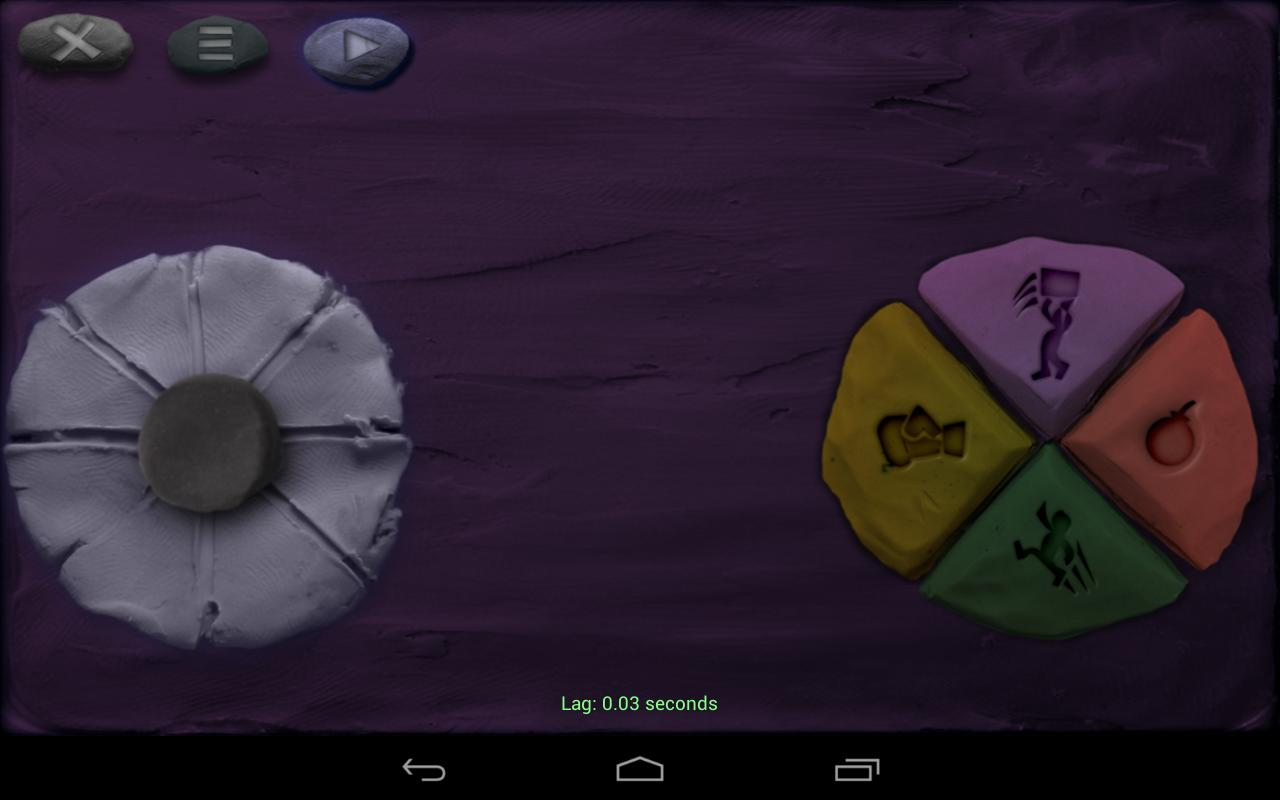
\includegraphics[width=1\textwidth]{figures/controlscheme/onscreen_control}
\caption{Bombsquad game screen, \url{http://www.froemling.net/wp-content/uploads/2014/04/IMG_1088.jpg}}
\end{figure}

The great thing about this control scheme is that it is compact, easy to use, and allows for focus on the gameplay it self, rather than making sure you are bashing the right buttons when you want to.

\subsection*{Heroes of the Order and Chaos}\label{sec:modules:controlscheme:hoftoac}
Heroes of the Order and Chaos\cite{hotoacGP} has the same movement scheme as BombSquad. 
Where it differs from BombSquad is in the actions-interface.
It is placed in the right side of the screen as in BombSquad, however, there are quite a few more actions than the four which BombSquad uses.
It includes 4 useable abilities along the right side of the screen, two useable abilities along the bottom of the screen, an \emph{attack} button and a \emph{change target} button.
\begin{figure}[H]
\centering
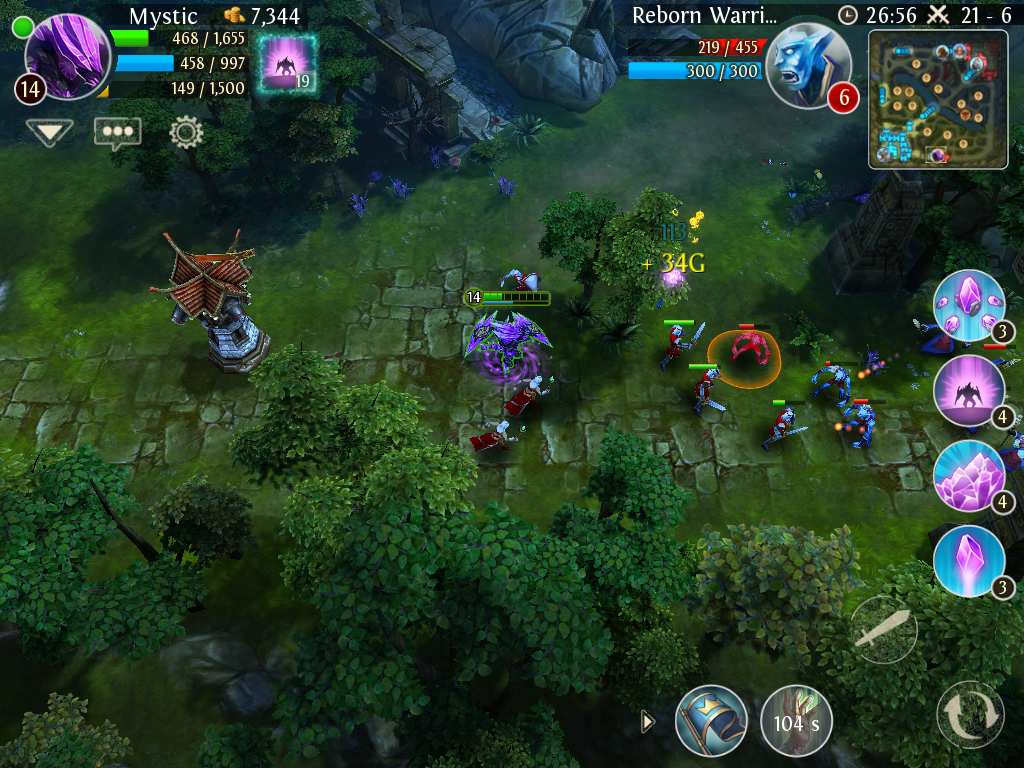
\includegraphics[width=1\textwidth]{figures/controlscheme/hotoac_control}
\caption{Heroes of the Order and Chaos control interface \url{http://3.bp.blogspot.com/-EQUyarxR56U/ULdIChk_LhI/AAAAAAAAArs/73MwPMoDhnI/s1600/IMG_3227.PNG}}
\end{figure}

The placement of the action buttons make it such that you don't accidentally hit the wrong buttons. 
There are quite a few input buttons though, so it takes a bit longer getting used to than the BombSquad interface. 
The buttons are also grouped such that the buttons you usually press in the same situations are at the same place. 
Further some in-game logic has been added such that some of the buttons wont always require pressing (such as attack), and some will queue if pressed in succession without the first action being finished.

\subsection{Gamepad controls}\label{sec:modules:controlscheme:gamepad:controls}
Using a gamepad to play the game is rather intuitive. Moving is done using the left thumb-stick, and aiming is done using the right thumbstick, much like in other games.
Due to the fact a gamepad has many buttons, we can bind shooting, aiming and actions to their own buttons. 
For navigating the menus, each menu item will be highlighted. The menu item is selected by clicking a button the the gamepad.
This is similar to the way most game menus are handled on a gamepad, and the control scheme is close to what shooting games normally use.

\subsection{Controls}
Given that we are trying to replicate a gamepad on a touch device, we follow a similar pattern as described in section \ref{sec:modules:controlscheme:gamepad:controls}. The inherit issue, however, is that  there is only one input option which is the screen. 
Two thumbsticks are present in the GUI on touch devices, the left one controlling movement, similar to \textit{BombSquad}, see section \ref{sec:modules:controlscheme:bombsquad}, and the right one controlling aim, see figure \ref{sec:modules:controlscheme:touch:controls:ui}.
In order to prevent cluttering the game-screen with a lot of input items, there is no button to shoot. If you aim in any direction, the character will shoot automatically. Similarly the character will also reload  automatically when it runs out of bullets. A button for reloading has been prioritized though, as some times you may want to reload before you actually run out of ammunition.
Contextual actions such as crafting will automatically show if you go near the ''crafting table'', rather than having a designated button for it. On other control-schemes it will require a button to be pressed in order to show.
Menus are navigated by performing a touch on the menu buttons. 

Figure \ref{sec:modules:controlscheme:prototype} shows the envisioned layout of the touch interface, and figure \ref{sec:modules:controlscheme:touch:controls:ui} shows the implemented layout from the game.
\begin{figure}[H]
\centering
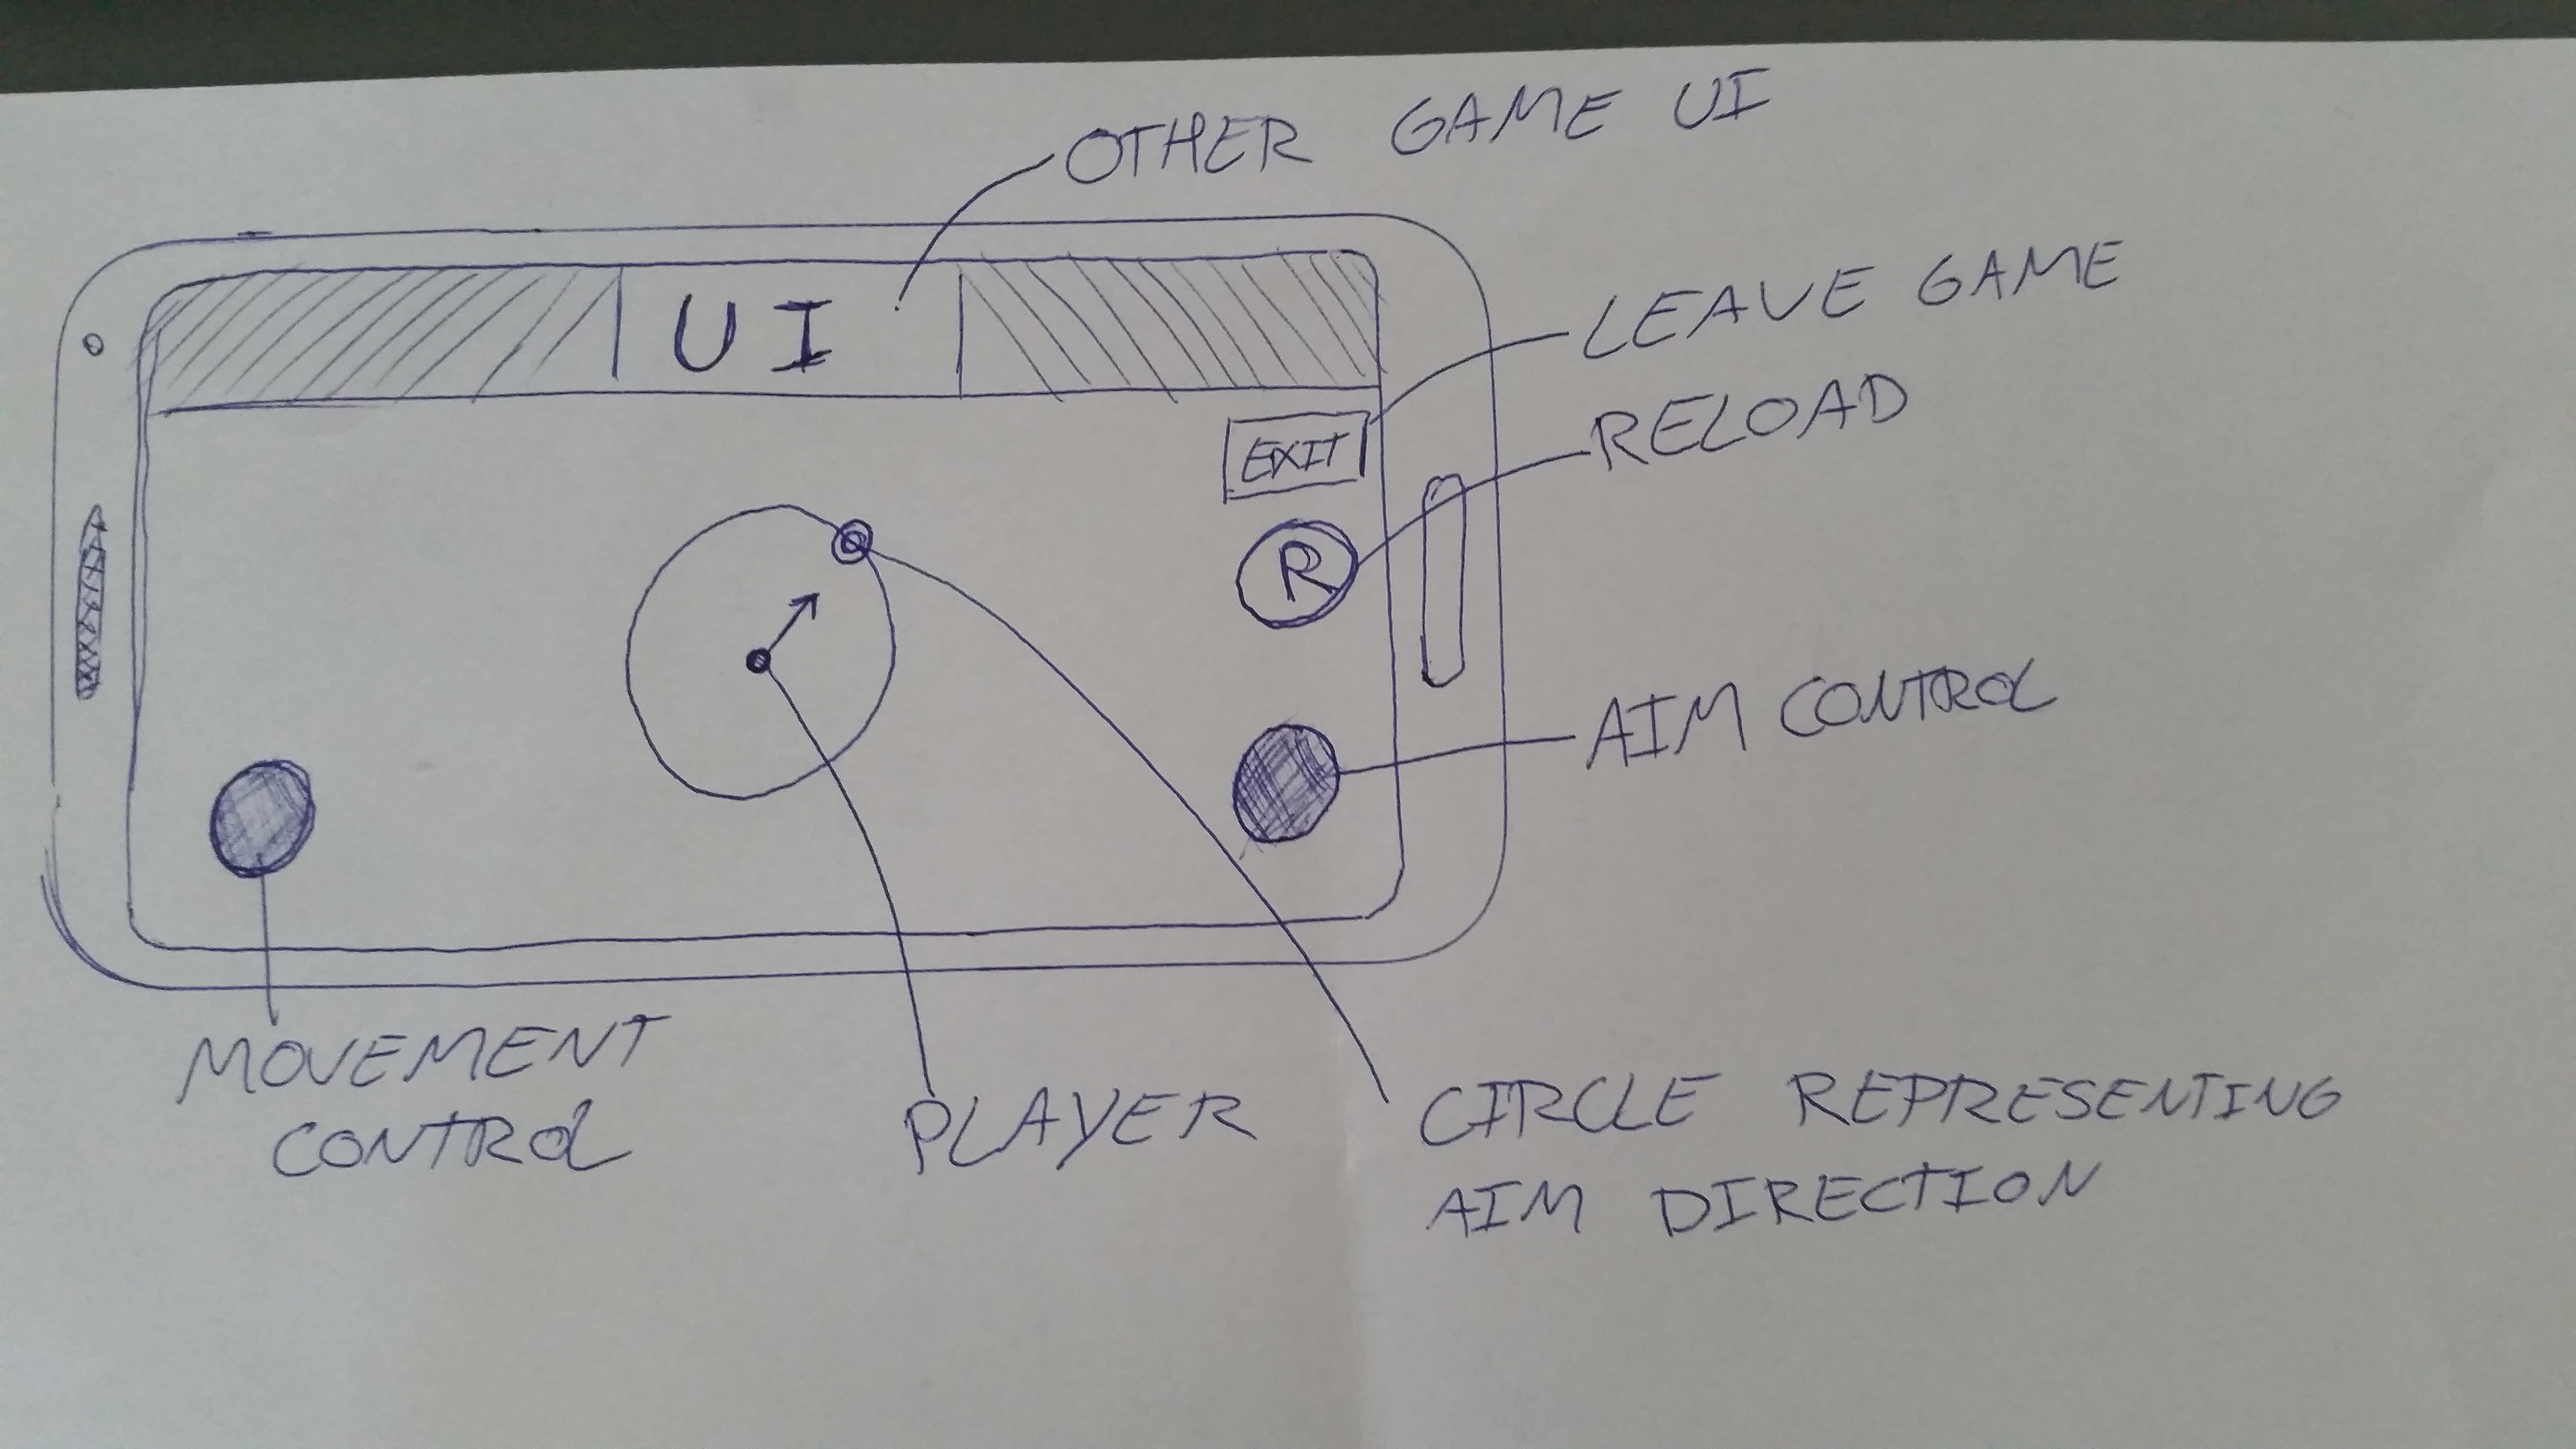
\includegraphics[width=.75\textwidth]{figures/controlscheme/prototype}
\caption{Papir visualization of the game control scheme.}
\label{sec:modules:controlscheme:prototype}
\end{figure}

\begin{figure}[H]
\centering
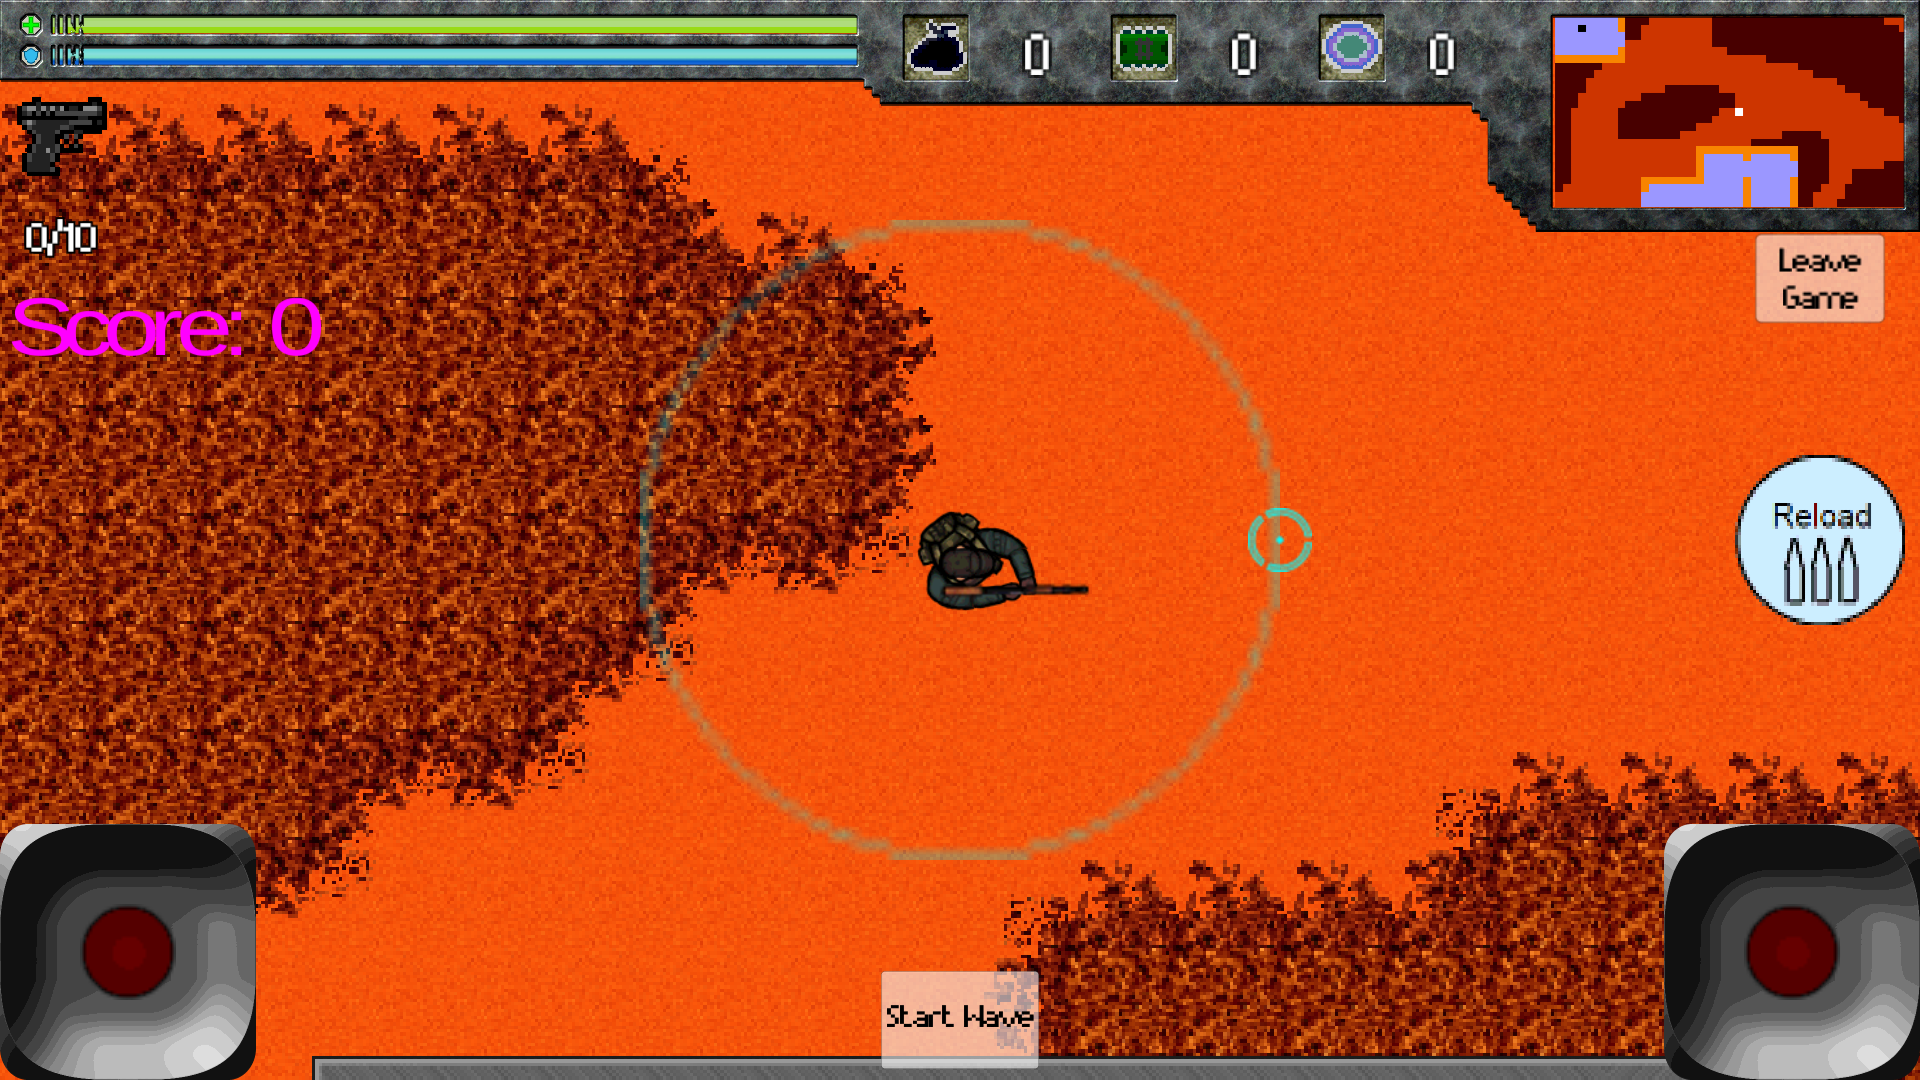
\includegraphics[width=.75\textwidth]{figures/controlscheme/ui}
\caption{UI for the game during development stages. You can see the GUI thumbsticks as well as some of the buttons.}
\label{sec:modules:controlscheme:touch:controls:ui}
\end{figure}